% sections/ml_inference.tex

\section{Multi-Runtime ML Inference}
\label{sec:ml_inference}

The routing system requires low-latency ML inference for signal extraction, classification, and embedding computation---all on the critical path of every request.
We describe the multi-runtime architecture that addresses the tension between inference speed, hardware flexibility, and model diversity.

\subsection{Design Constraints}

Three constraints shape the inference architecture:
\begin{enumerate}
  \item \textbf{Latency}: Signal extraction must complete within the tail latency budget of the routing system (target: $<$100\,ms for all signals combined).
  \item \textbf{Hardware heterogeneity}: Deployments range from GPU-equipped data centers to CPU-only edge nodes.
  \item \textbf{Model diversity}: Different tasks require different model architectures (sequence classification, token classification, NLI, embeddings, MLP).
\end{enumerate}

\subsection{Four-Runtime Architecture}

We implement four inference runtimes, each optimized for different hardware and task profiles, all exposed to the Go routing process via C FFI and CGo (\Cref{fig:ml_runtimes}):

\begin{table}[h]
\centering
\caption{Inference runtime characteristics}
\label{tab:runtimes}
\begin{tabular}{llll}
\toprule
\textbf{Runtime} & \textbf{Target Hardware} & \textbf{Tasks} & \textbf{Framework} \\
\midrule
Candle       & GPU (CUDA), CPU & Classification, LoRA, MLP & HF Candle~\cite{candleml2024} \\
Linfa        & CPU only        & KNN, KMeans, SVM         & Linfa~\cite{linfa2024} \\
ONNX RT      & CPU, GPU        & Embeddings               & ONNX Runtime~\cite{onnxruntime2024} \\
NLP Binding  & CPU only        & BM25, N-gram matching    & bm25 + ngrammatic (Rust) \\
\bottomrule
\end{tabular}
\end{table}

All runtimes are compiled as Rust shared libraries (\texttt{.so}/\texttt{.a}) and linked to the Go routing process via CGo.
This eliminates Python runtime overhead, GIL contention, and inter-process communication latency that would arise from serving models in separate Python processes.

\begin{figure*}[ht]
\centering
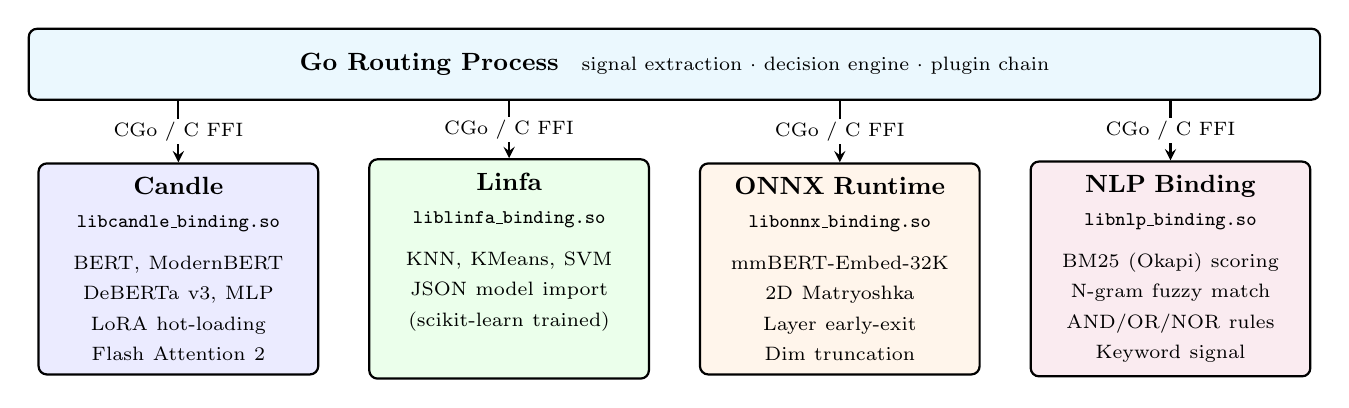
\begin{tikzpicture}[
  gobox/.style={rectangle, draw, thick, rounded corners=3pt, fill=cyan!8,
                minimum width=16.4cm, minimum height=0.9cm, align=center,
                inner sep=5pt, font=\small},
  rt/.style={rectangle, draw, thick, rounded corners=3pt,
             text width=3.2cm, align=center, inner sep=5pt, font=\small},
  arr/.style={->, >=stealth, thick},
  ffi/.style={font=\scriptsize, midway, fill=white, inner sep=1pt},
]

% Go process
\node[gobox] (go) at (0, 2.6)
  {\textbf{Go Routing Process}\;\;
   {\scriptsize signal extraction $\cdot$ decision engine $\cdot$ plugin chain}};

% Four runtimes -- spaced at 4.2cm intervals
\node[rt, fill=blue!8] (candle) at (-6.3, 0) {%
  \textbf{Candle}\\[1pt]
  {\scriptsize\texttt{libcandle\_binding.so}}\\[4pt]
  {\scriptsize BERT, ModernBERT}\\
  {\scriptsize DeBERTa v3, MLP}\\
  {\scriptsize LoRA hot-loading}\\
  {\scriptsize Flash Attention 2}};

\node[rt, fill=green!8] (linfa) at (-2.1, 0) {%
  \textbf{Linfa}\\[1pt]
  {\scriptsize\texttt{liblinfa\_binding.so}}\\[4pt]
  {\scriptsize KNN, KMeans, SVM}\\
  {\scriptsize JSON model import}\\
  {\scriptsize (scikit-learn trained)}\\[3pt]~};

\node[rt, fill=orange!8] (onnx) at (2.1, 0) {%
  \textbf{ONNX Runtime}\\[1pt]
  {\scriptsize\texttt{libonnx\_binding.so}}\\[4pt]
  {\scriptsize mmBERT-Embed-32K}\\
  {\scriptsize 2D Matryoshka}\\
  {\scriptsize Layer early-exit}\\
  {\scriptsize Dim truncation}};

\node[rt, fill=purple!8] (nlp) at (6.3, 0) {%
  \textbf{NLP Binding}\\[1pt]
  {\scriptsize\texttt{libnlp\_binding.so}}\\[4pt]
  {\scriptsize BM25 (Okapi) scoring}\\
  {\scriptsize N-gram fuzzy match}\\
  {\scriptsize AND/OR/NOR rules}\\
  {\scriptsize Keyword signal}};

% CGo/FFI arrows
\draw[arr] (go.south -| candle) -- node[ffi] {CGo / C FFI} (candle.north);
\draw[arr] (go.south -| linfa)  -- node[ffi] {CGo / C FFI} (linfa.north);
\draw[arr] (go.south -| onnx)   -- node[ffi] {CGo / C FFI} (onnx.north);
\draw[arr] (go.south -| nlp)    -- node[ffi] {CGo / C FFI} (nlp.north);

\end{tikzpicture}
\caption{Four-runtime ML inference architecture. The Go routing process links to four Rust shared libraries via CGo/C~FFI. Each runtime is specialized for a different class of ML workload, avoiding Python overhead on the critical path.}
\label{fig:ml_runtimes}
\end{figure*}

\subsection{Candle Runtime: GPU-Accelerated Classification}

The Candle runtime handles all transformer-based classification tasks, including LoRA adapter loading and inference (\Cref{sec:lora_mom}).

\textbf{Supported architectures.}
BERT~\cite{devlin2019bert}, ModernBERT~\cite{warner2024modernbert} (with Flash Attention and GeGLU), mmBERT-32K (YaRN RoPE for 32K context), DeBERTa v3 (NLI), and feed-forward MLPs (model selection).

\textbf{Optimization features.}
Flash Attention 2 kernels reduce attention memory from $O(n^2)$ to $O(n)$ and improve throughput.
Optional Intel MKL integration for CPU deployments.
LoRA adapter hot-loading enables runtime model updates without restart.

\subsection{ModernBERT-base-32k: Extended Context Window}

The Candle runtime supports ModernBERT-base-32k, extending the context window from 512 tokens (BERT-base) to 32,768 tokens via YaRN (Yet another RoPE extensioN) scaling~\cite{peng2023yarn}.
This enables signal extraction from long documents and multi-turn conversations that exceed the traditional 512-token limit.

\textbf{Architecture and scaling.}
ModernBERT-base-32k uses Rotary Position Embeddings (RoPE) with YaRN scaling to extend the base model's 8,192-token context to 32K tokens.
The model maintains compatibility with existing LoRA adapters trained on BERT-base, enabling seamless migration without retraining classifier heads.
Flash Attention 2 provides memory-efficient attention computation, reducing memory requirements from $O(n^2)$ to $O(n)$ for long sequences.

\textbf{Performance characteristics.}
Empirical benchmarks on NVIDIA L4 GPU (23GB VRAM) demonstrate reliable performance for context lengths up to 8K tokens:
\begin{itemize}[leftmargin=*]
  \item \textbf{1K tokens}: p50 latency $\sim$94\,ms at C=1, $\sim$970\,ms at C=10 (100\% success rate)
  \item \textbf{4K tokens}: p50 latency $\sim$955\,ms at C=1, $\sim$9,389\,ms at C=10 (93\% success rate, 7 OOM errors)
  \item \textbf{8K tokens}: p50 latency $\sim$3,525\,ms at C=1, fails at C=10 due to insufficient GPU memory
\end{itemize}
For sequences exceeding 32K tokens, automatic chunking with configurable overlap (default 128 tokens) enables processing of arbitrarily long documents while preserving context continuity.

\textbf{Hardware requirements.}
Production deployments for 1K--8K tokens require a GPU with $\geq$23GB VRAM (e.g., NVIDIA L4, A10G).
Full 32K token support and high concurrency (C=50+) require $\geq$40GB VRAM (e.g., NVIDIA A100).
CPU inference is supported but incurs significant latency penalties ($\sim$45$\times$ slower for 512 tokens).

\textbf{Backward compatibility.}
The integration maintains full backward compatibility with existing BERT-base workflows.
Sequences $\leq$512 tokens exhibit no performance degradation, and existing LoRA adapters (domain classification, PII detection, jailbreak detection) function without modification.

\subsection{Linfa Runtime: CPU ML Inference}

Classical ML model selection algorithms (KNN, KMeans, SVM) are served by the Linfa runtime.
These algorithms operate on pre-computed feature vectors and do not require GPU acceleration, making Linfa's lightweight CPU implementation ideal.

\textbf{Training-inference split.}
Models are trained in Python (scikit-learn, custom implementations) and serialized to JSON.
The Rust runtime loads serialized models at startup and performs inference-only computation.
This decouples the training environment (Python, GPU-optional) from the inference environment (Rust, CPU-only), enabling simpler deployment.

\subsection{ONNX Runtime: Efficient Embeddings}

Embedding computation is served by ONNX Runtime, optimized for the mmBERT-Embed-32K model with 2D Matryoshka representation learning~\cite{kusupati2022matryoshka}.

\textbf{2D Matryoshka trade-offs.}
The architecture supports two-dimensional quality-latency trade-offs:
\begin{itemize}[leftmargin=*]
  \item \textbf{Layer early-exit}: Extract embeddings from intermediate layers (6, 11, 16, or 22 out of 22), achieving $\sim$3--4$\times$ speedup at layer 6 with modest quality degradation.
  \item \textbf{Dimension truncation}: Reduce embedding dimension from 768 to 64, 128, 256, or 512, reducing memory and computation for similarity search.
\end{itemize}

For the $\sim$150M parameter embedding model, CPU inference with 2D Matryoshka (layer 11, dimension 256) achieves latency comparable to GPU inference on the full model, making GPU optional for embedding computation.

\subsection{NLP Binding Runtime: Keyword Classification}

The NLP Binding runtime handles BM25 and N-gram keyword matching for the keyword signal type, complementing the ML-based classifiers served by Candle.
Unlike the neural runtimes, NLP Binding implements statistical text matching algorithms that require no model weights or GPU:

\textbf{BM25 (Okapi).}
The BM25 classifier uses the Rust \texttt{bm25} crate to compute term-frequency--inverse-document-frequency scores between query text and keyword rules.
Each rule specifies a set of keywords, a Boolean operator (AND/OR/NOR), a score threshold, and case-sensitivity.
A keyword is considered matched when its BM25 relevance score exceeds the configured threshold.

\textbf{N-gram fuzzy matching.}
The N-gram classifier uses the \texttt{ngrammatic} crate to perform fuzzy string matching via character n-gram overlap (default: trigrams, Jaccard similarity).
This enables matching despite typos and morphological variation---e.g., \texttt{"urgnet"} matches the keyword \texttt{"urgent"} when the similarity exceeds the configured threshold.

\textbf{FFI design.}
The binding follows the same conventions as \texttt{candle-binding}: Rust \texttt{\#[repr(C)]} structs, \texttt{\#[no\_mangle] pub extern "C" fn} exports, CString-based string passing, and explicit free functions for Rust-allocated memory.
The Go side wraps each classifier as a handle-based API (\texttt{BM25Classifier}, \texttt{NgramClassifier}) with lifecycle management (\texttt{New}, \texttt{AddRule}, \texttt{Classify}, \texttt{Free}).
Thread safety is provided by Rust \texttt{Mutex}-guarded global state with atomic handle generation.

\subsection{Runtime Selection Strategy}

The routing system selects runtimes based on deployment configuration.
The NLP Binding is always active when keyword signal rules use \texttt{bm25} or \texttt{ngram} methods:
\begin{itemize}[leftmargin=*]
  \item \textbf{GPU available}: Candle (classification + LoRA) + ONNX (embeddings) + Linfa (ML selection) + NLP Binding (keyword).
  \item \textbf{CPU only}: Candle with MKL (classification) + ONNX with early-exit (embeddings) + Linfa (ML selection) + NLP Binding (keyword).
  \item \textbf{Minimal}: ONNX (embeddings) + Linfa (ML selection) + NLP Binding (keyword), with classification delegated to external vLLM-served models.
\end{itemize}
